\begin{center}
    \begin{circuitikz}
        % Draw a voltage source from 0 to 5V
        \draw (0,0) to [american voltage source, voltage dir=RP, v=$V_{in}$] (0,4);
        \draw (0,4) to [R, l=$100\Omega$] (\linewidth/4,4);
        \draw (\linewidth/4,4) to [L, l=$10\text{mH}$] (\linewidth/2,4);
        % Draw a C that connects to the voltage in
        \draw (\linewidth/2,4) to [C, l=$6\text{n}8\text{F}$] (\linewidth/2,0);
        \draw (\linewidth/2,0) to (0,0);
    \end{circuitikz}
\end{center}

The second order differential equation for this RLC series circuit is solved by remembering that
\begin{equation}
    i = i_C = C\frac{dV_c}{d_t}
\end{equation}
Taking this into account, our mesh will be defined as follows:
\begin{equation}
    V_{in} = V_R + V_C + V_L
\end{equation}
Where we define each component by their respective relations:
\begin{equation}
    \begin{gathered}
        V_L = L\frac{di}{dt} \\
        V_R = iR \\
        i_C = C\frac{dV_C}{dt}
    \end{gathered}
\end{equation}
Substituting these relations into the mesh equation, we get the following:
\begin{equation}
    V_{in} = LC\frac{d^2V_C}{dt^2} + RC\frac{dV_C}{dt} + V_C
\end{equation}
Which is a second-order differential equation. We can define the following constants:
\begin{equation}
    a_2 = LC, \quad a_1 = RC, \quad a_0 = 1
\end{equation}
Subsequently, we can find that the proper form of the differential equation by recalling that for a second-order differential equation, we have the following:
\begin{equation}
    \zeta = \frac{a_1}{2\sqrt{a_0a_2}}, \quad \omega_n = \sqrt{\frac{a_0}{a_2}}
\end{equation}
Using {\bf MATLAB}, we can verify the behaviour of the circuit.
\begin{verbatim}
% For the case where R = 100Ohm, C = 6.8nF and L=10mH
R = 100;
C = 6.8E-9;
L = 10E-3;

zeta = R/2 * sqrt(C/L); % approximately 0.0412, so underdamped
w_n = 1/sqrt(L*C);
w_d = w_n * sqrt(1 - zeta^2);

\end{verbatim}
We find that
\begin{equation}
    \zeta = 0.0412, \quad \omega_n = 1.2127\times10^5 \text{rad/s} \quad \omega_d = 1.2116\times10^5 \text{rad/s}
\end{equation}
Which serves to tell us that the circuit is underdamped.
To identify the initial conditions $C_1$ and $C_2$ of the circuit, knowing that we have an underdamped circuit, we can use the following relations for the complete response, where we know that:

\begin{equation}
    y_t(t) = y_h(t) + y_f(t)
\end{equation}

Where $y_h(t)$ is the homogeneous response and $y_f(t)$ is the forced response.

\begin{equation}
    y(t) = e^{-\zeta \omega_n t}\left(C_1\cos(\omega_d t) + C_2\sin(\omega_d t)\right) + V_{in}
\end{equation}

Where $V_{in}$ in our case is simply 1V. We know that at $t=0$, the voltage over the capacitor is 0V.

\begin{equation}
    y(0) = C_1 + V_{in} \implies y(0) = C_1 + V_{in} \implies C_1 = -V_{in} = -1V.
\end{equation}
Consider that the change over the capacitor is also 0V at immediately $t=0$,
it follows that for:
\begin{equation}
    \frac{dy}{dt} = e^{-\zeta \omega_n t} \left(C_2 \omega_d \cos(\omega_d t) - C_1 \omega_d \sin(\omega_d t)\right) - \omega_n \zeta e^{-\zeta \omega_n t} \left(C_1\cos(\omega_d t) + C_2\sin(\omega_d t)\right)
\end{equation}
Evaluated at $t=0$, we get:
\begin{equation}
    \begin{gathered}
        \frac{dy}{dt}(0) = C_2 \omega_d - \omega_n \zeta C_1 \\
        0 = C_2 \omega_d - \omega_n \zeta C_1 \\
        C_2 = - \frac{\omega_n}{\omega_d} \zeta
    \end{gathered}
\end{equation}
Which, using {\bf MATLAB} we can verify that $C_2 = -0.0413$.
\begin{verbatim}
C1 = -1;
C2 = -(w_n/w_d) * zeta; % -0.0413    
\end{verbatim}

Plotting the data using {\bf MATLAB} we get the following for the voltage over the capacitor:

\begin{figure}[H]
    \centering
    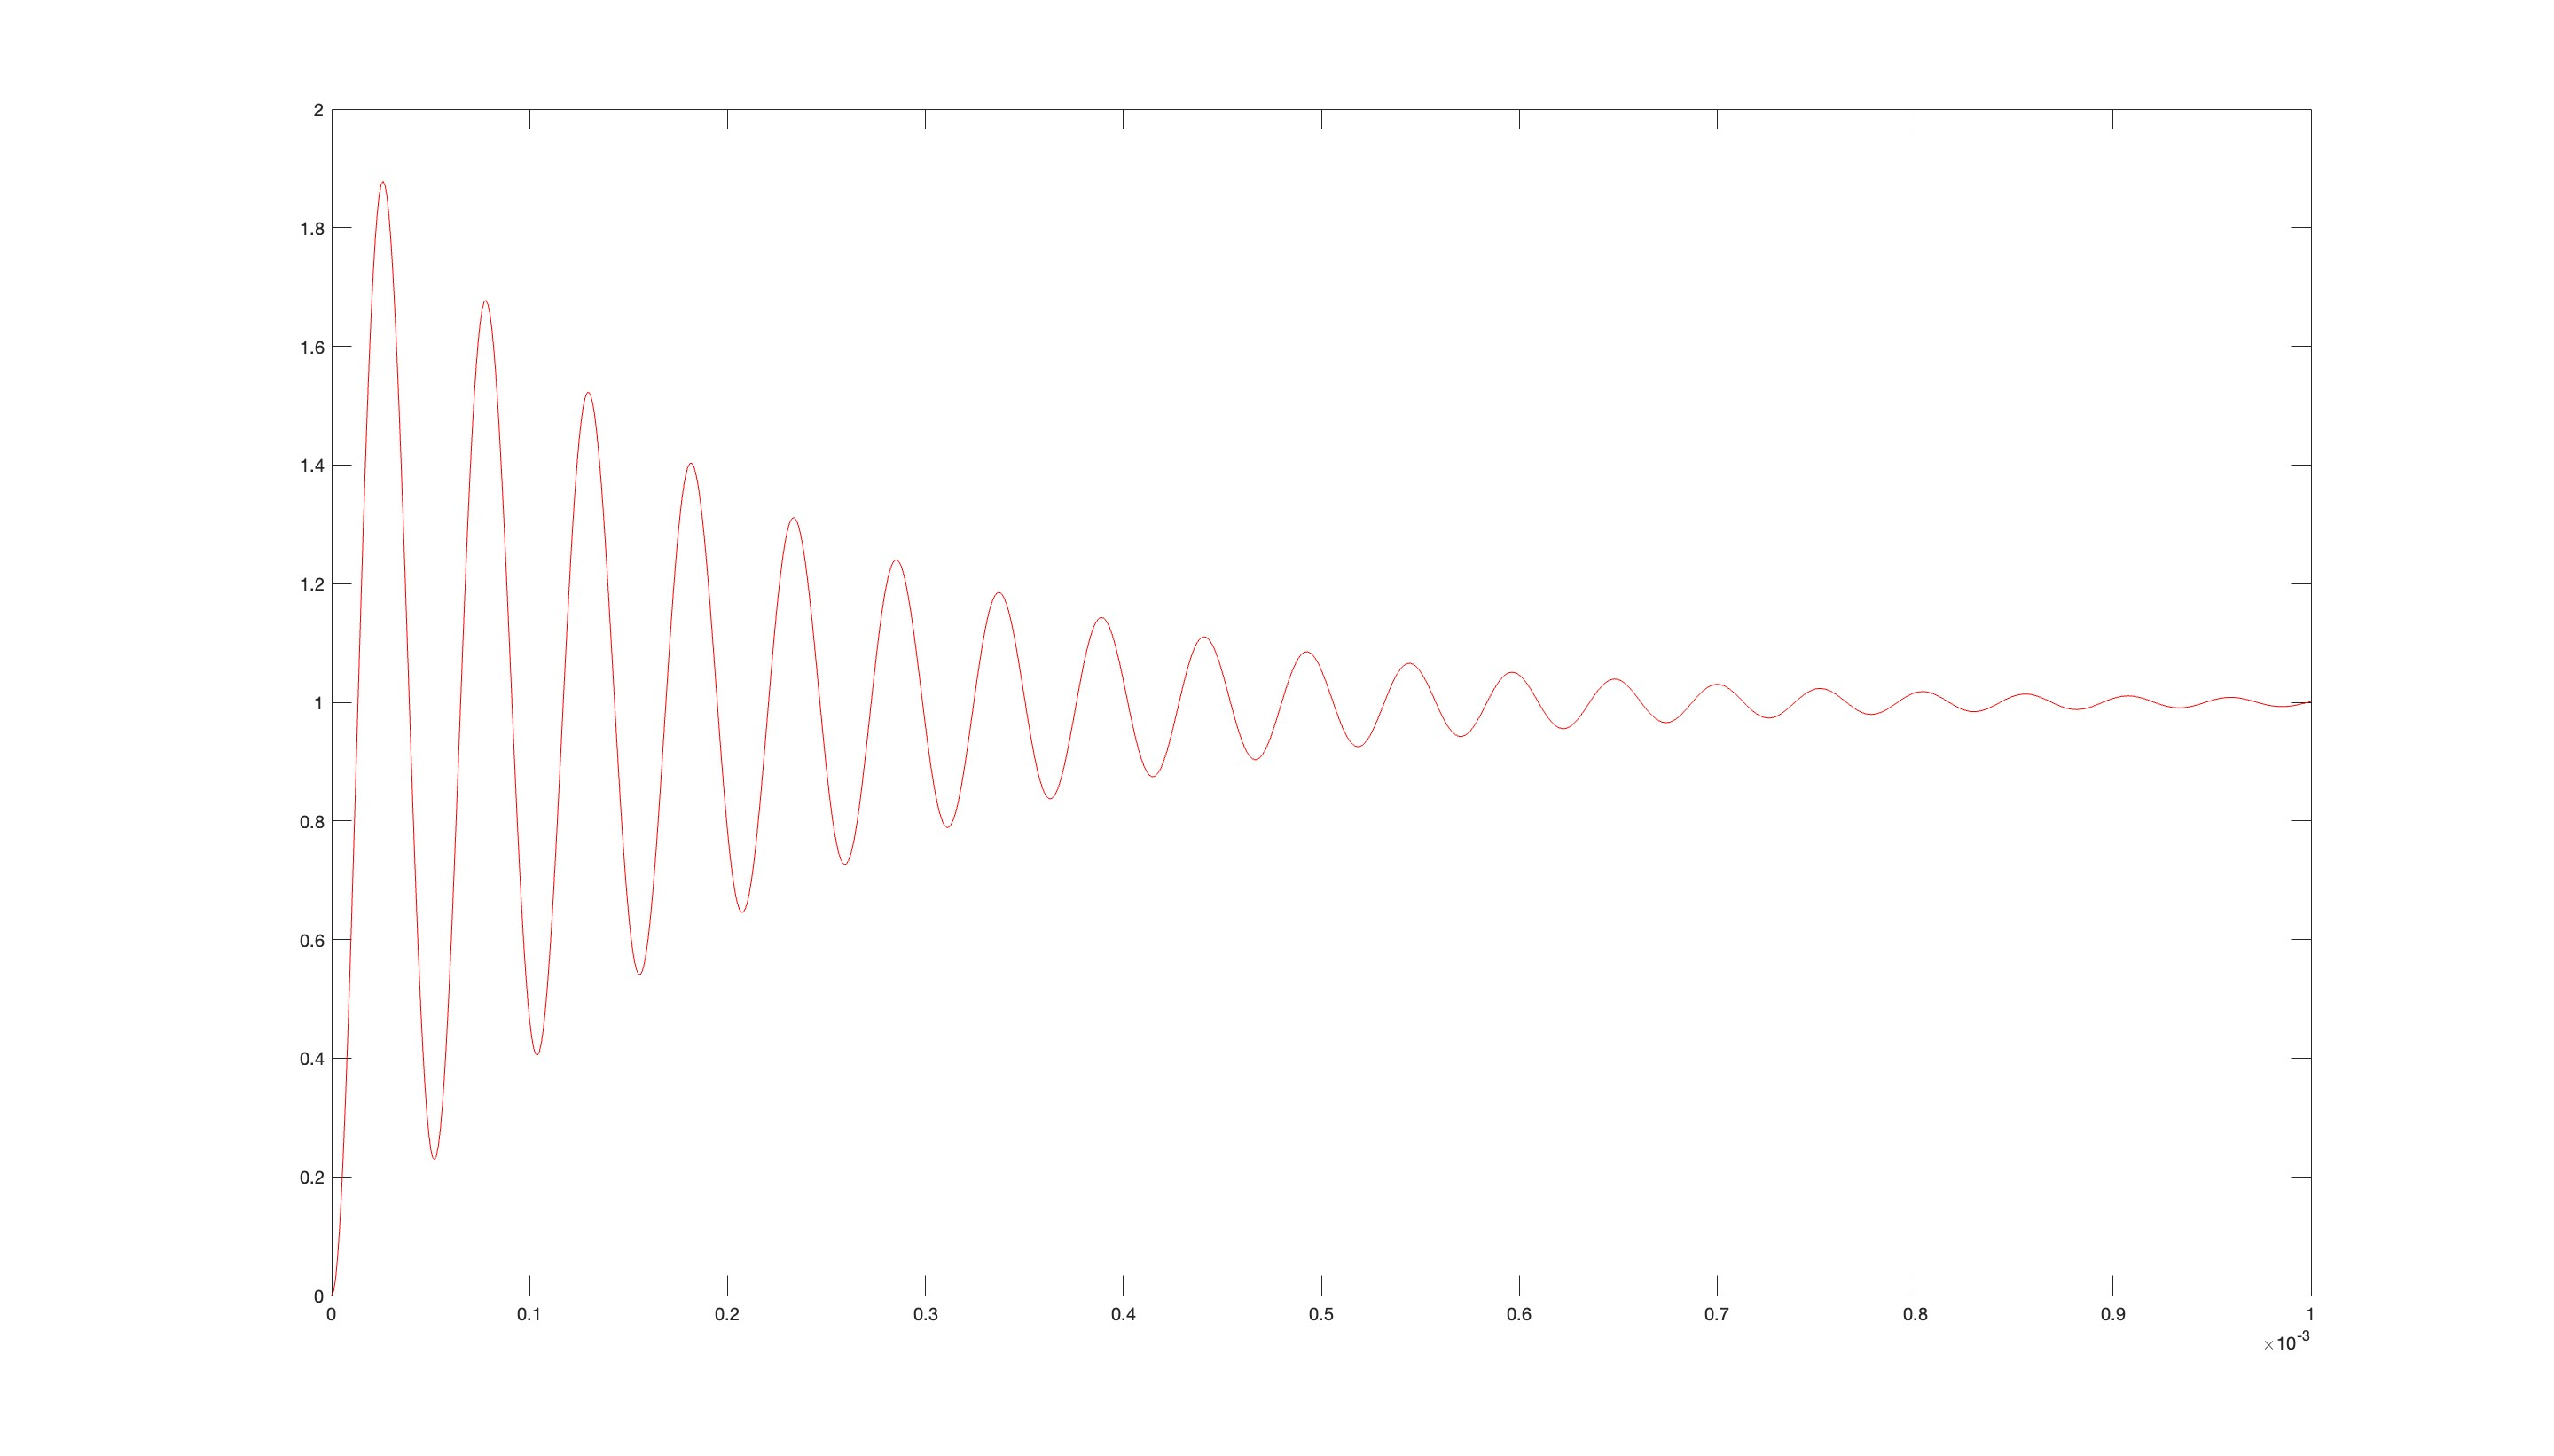
\includegraphics[width=\linewidth]{images/evaluation_vc.jpg}
    \caption{Voltage over the capacitor}
    \label{fig:evaluation_vc}
\end{figure}
Confirming our results, we can that the voltage over the capacitor displays underdamped behaviour.

In order to get {\bf critically damped} behaviour, we know that $\zeta = 1$. We can use the following relation to find the optimal resistance to make $\zeta$ go to $1$.

\begin{equation}
    \begin{gathered}
        \zeta = \frac{R}{2} \sqrt{C/L} \\
        \text{Knowing that $\zeta = 1$} \\
        R = \frac{2}{\sqrt{C/L}} \\
    \end{gathered}
\end{equation}

Now that we have a critically damped circuit, we can find the initial
conditions $C_1$ and $C_2$ by knowing that the general solution
for a critically damped circuit is given

\begin{equation}
    y(t) = e^{-\zeta \omega_n t}\left(C_1 + C_2 t\right) + V_{in}
\end{equation}
Knowing that $V_{in}$ is 1V, we can find the initial condition $C_1$ straightforwardly:
\begin{equation}
    y(0) = C_1 + V_{in} \implies C_1 = -V_{in} = -1V.
\end{equation}
Finding $C_1$, we can now move towards finding $C_2$ by taking the derivative
of the general solution for this critically damped circuit:
\begin{equation}
    \frac{dy}{dt} = -\zeta \omega_n C_1 e^{-\zeta \omega_n t} - \zeta w_n C_2 t e^{-\zeta \omega_n t} + C_2 e^{-\zeta \omega_n t}
\end{equation}

Evaluating this at $t=0$, and knowing $\zeta = 1$, we get:
\begin{equation}
    0 = -\zeta \omega_n C_1 + C_2 \implies C_2 = \zeta \omega_n C_1 \implies C_2 = -\omega_n
\end{equation}

Subsequently, we arrive at the conclusion that $C_2 = -1.2127\times10^5$.
Plotting the data using {\bf MATLAB} we get the following for the voltage over the capacitor in both the critically damped and underdamped cases:

\begin{figure}[H]
    \centering
    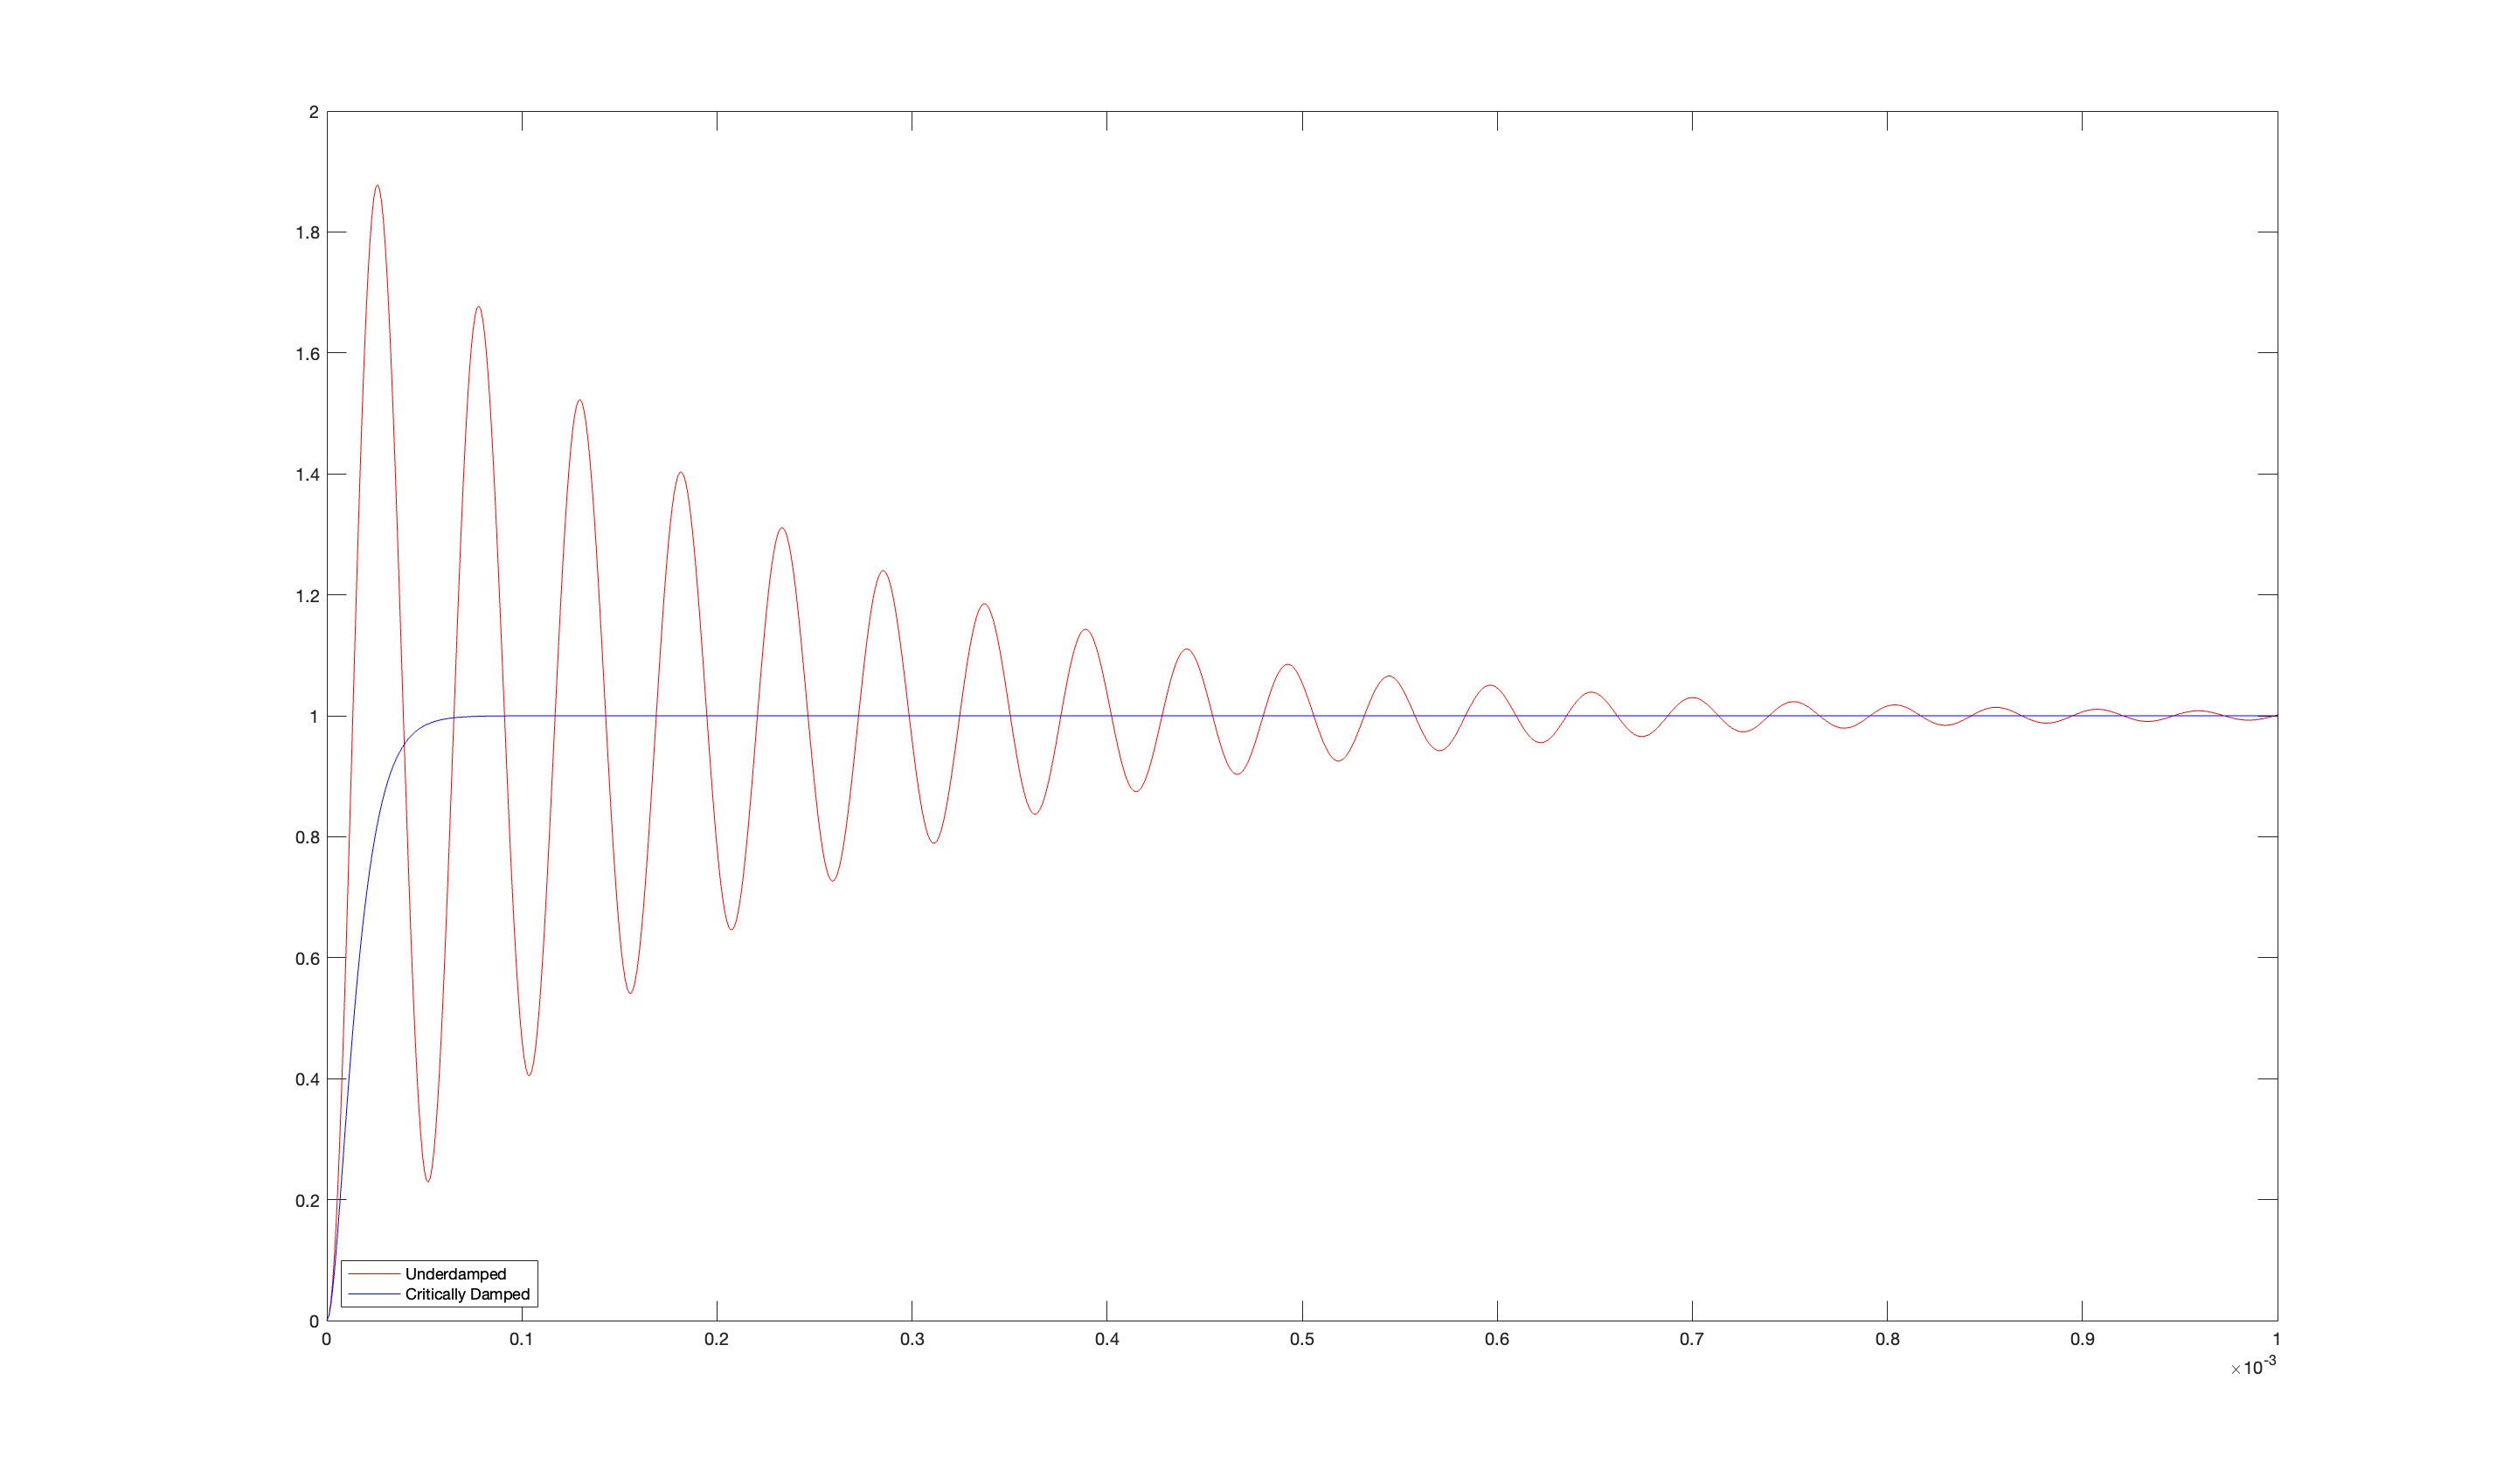
\includegraphics[width=\linewidth]{images/evaluation_vc_full.png}
    \caption{Voltage over the capacitor for both underdamped and critically damped cases}
    \label{fig:evaluation_vc_crit}
\end{figure}

The {\bf MATLAB} code used to generate both of these plots is provided below:
\newpage
\begin{verbatim}
%% Part 1:
clear

% For the case where R = 100Ohm, C = 6.8nF and L=10mH
R = 100;
C = 6.8E-9;
L = 10E-3;

zeta = R/2 * sqrt(C/L); % approximately 0.0412, so underdamped
w_n = 1/sqrt(L*C);
w_d = w_n * sqrt(1 - zeta^2);

% We know that the circuit is underdamped because zeta < 1

% We obtained C1 = -1, C2 = -(w_n/w_d) * zeta
C1 = -1;
C2 = -(w_n/w_d) * zeta;

t = 0:1E-6:1E-3;
y = exp(-zeta * w_n .* t) .* (C1*cos(w_d.*t) + C2 * sin(w_d.*t)) + 1;
plot(t, y, 'red');

hold on

%% Critically damped

% For the critically damped case:
R = 2 * (1 / sqrt(C/L));
zeta = R/2 * sqrt(C/L);
w_n = 1/sqrt(L*C);

% We obtained that C1 = -1, and C2 = -w_n.
C2 = -w_n;
C1 = -1;
y = (C1*exp(-zeta * w_n .* t) + C2.*t.*exp(-zeta * w_n .* t)) + 1;
plot(t, y, 'blue');

legend({'Underdamped','Critically Damped'},'Location','southwest')
\end{verbatim}

Compared to the results we obtained in the laboratory, we can see that the results are very similar, with the only difference being that the voltage over the capacitor in the laboratory when the resistance is at its optimum theoretical value of
$2375\Omega$, where $\zeta$ becomes $1$ and thereby gives us critical damping, gives us a slightly more over-damped response than playing around with the resistance in the R-Decade, which got us a resistance of around $1905\Omega$. This is because of the internal resistance of the R-Decade, which is not taken into account in the theoretical calculations. Furthermore, the theoretical calculations do not take into account the resistance of the wires, the resistance of the capacitor, nor the resistance of the inductor, which all contribute to the overall resistance of the circuit. This is why the theoretical calculations do not match the laboratory results exactly.